\documentclass[../report.tex]{subfiles}
\begin{document}
\section{Technologies du projet}
Cette section présente les différentes technologies liées au projet, en fournissant pour chacune une description ainsi que leur rôle dans le projet.
\subsection{GraalVM}
GraalVM est une machine virtuelle universelle, conçue pour permettre l'exécution d'un grand nombre de langages de programmation différents et de faciliter la création de nouveaux langages. GraalVM essaie de résoudre les problèmes liés à la création d'un nouveau langage : fournir un débogueur, un compilateur et d'autres outils...\\
GraalVM permet également l'interopérabilité entre différents langages : on peut par exemple écrire une méthode en Javascript et l'invoquer dans un code source Python.

Du côté technique, GraalVM est basé sur la \textit{Java Virtual Machine}, mais avec de nombreuses modifications sur le compilateur à la volée permettant d'augmenter les performances. GraalVM est également capable de créer des images natives compilées avant l'exécution, afin de s'affranchir du besoin d'avoir une machine virtuelle Java disponible.

Le rôle de GraalVM dans ce projet est de fournir la plateforme permettant de lancer l'application finale. À noter qu'il est également possible de lancer l'application sur une JVM classique, mais les performances sont réduites sans les capacités d'optimisations et de compilation à la volée de GraalVM.
\subsection{Truffle}
Truffle est une librairie Java open source permettant de réaliser des interpréteurs pour des langages de programmation. C'est la librairie qui permet de faire le lien entre le langage de programmation et les capacités de GraalVM. Ce lien donne toute sa puissance à la suite de technologies, car il permet en écrivant uniquement un interpréteur de bénéficier de performances proches d'un compilateur, et écrire un interpréteur est en général bien plus facile qu'écrire un compilateur.

Son rôle dans le projet est central : la majeure partie de l'implémentation se fait en utilisant l'API de Truffle.
\subsection{Prolog}
Prolog est un langage de programmation logique. Il permet de réaliser des programmes en utilisant une syntaxe déclarative plutôt que impérative. Prolog a été choisi en raison de l'absence d'implémentations de langages de programmation logique avec Truffle et GraalVM.

Prolog sert donc de base au projet pour lui donner une direction et un but. Son fonctionnement interne sera un élément central, vu qu'il s'agit de ce qui sera au final implémenté. En revanche, le langage en lui-même ne sera pas utilisé pour programmer des parties du projet, à part pour écrire des tests permettant de vérifier le fonctionnement de l'interpréteur.
\subsection{ANTLR}
ANTLR est un outil permettant de générer un lexer et un parser dans différents langages à partir d'un fichier décrivant la syntaxe du langage.

ANTLR sert à générer les fichiers Java permettant de parser un fichier Prolog et d'en ressortir les différents éléments.
\subsection{Java}
Java est le langage de programmation dans lequel sera réalisé le projet.
\subsection{Maven}
Maven est l'outil permettant de gérer le cycle de vie du projet Java, en gérant automatiquement les tests et la compilation, ainsi que les dépendances ou encore la génération du fichier JAR contenant l'application.
\subsection{Relations entre les technologies}
La figure \ref{fig:technologiesRelationship} schématise les différentes relations entre les technologies du projet.
\begin{figure}[h]
    \centering
    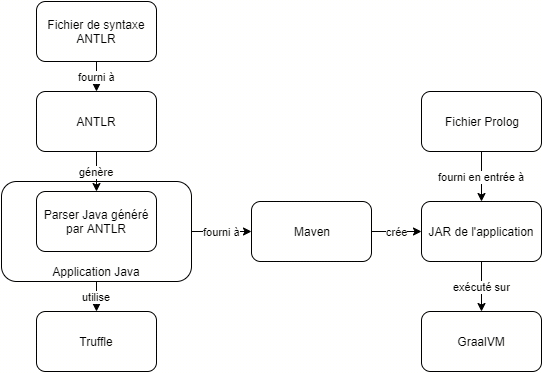
\includegraphics[width=0.75\textwidth]{techrelationshipdiagram.png}
    \caption{Relations entre les différentes technologies}
    \label{fig:technologiesRelationship}
\end{figure}
\end{document}